%%*************************************************************************
%% Legal Notice:
%% This code is offered as-is without any warranty either expressed or
%% implied; without even the implied warranty of MERCHANTABILITY or
%% FITNESS FOR A PARTICULAR PURPOSE! 
%% User assumes all risk.
%% In no event shall IEEE or any contributor to this code be liable for
%% any damages or losses, including, but not limited to, incidental,
%% consequential, or any other damages, resulting from the use or misuse
%% of any information contained here.
%%
%% All comments are the opinions of their respective authors and are not
%% necessarily endorsed by the IEEE.
%%
%% This work is distributed under the LaTeX Project Public License (LPPL)
%% ( http://www.latex-project.org/ ) version 1.3, and may be freely used,
%% distributed and modified. A copy of the LPPL, version 1.3, is included
%% in the base LaTeX documentation of all distributions of LaTeX released
%% 2003/12/01 or later.
%% Retain all contribution notices and credits.
%% ** Modified files should be clearly indicated as such, including  **
%% ** renaming them and changing author support contact information. **
%%
%% File list of work: IEEEtran.cls, IEEEtran_HOWTO.pdf, bare_adv.tex,
%%                    bare_conf.tex, bare_jrnl.tex, bare_jrnl_compsoc.tex
%%*************************************************************************

\documentclass[10pt, conference, compsocconf]{IEEEtran}

\usepackage{ucs}
\usepackage[utf8x]{inputenc}
\usepackage[english]{babel}
\usepackage{hyperref}     % use \url{http://$URL} or \href{http://$URL}{Name}
\usepackage{underscore}   % underscores need not be escaped
\usepackage{subfigure}
\usepackage{verbatim}
\usepackage{moreverb}
\usepackage{float}
\usepackage{booktabs}     % professional tables
\usepackage{listings}
\usepackage{color}
\usepackage{amsmath}
\usepackage{indentfirst}
\definecolor{darkgreen}{rgb}{0,0.4,0}
\lstset{language=C,captionpos=b,tabsize=3,frame=lines,keywordstyle=\color{blue},commentstyle=\color{darkgreen},stringstyle=\color{red},numbers=left,numberstyle=\tiny,numbersep=5pt,breaklines=true,showstringspaces=false,basicstyle=\footnotesize,emph={label}}

% Support for including graphics
\usepackage{graphicx}
\DeclareGraphicsExtensions{.pdf,.png,.jpg}
\graphicspath{{./src/images/}}

\begin{document}

\title{Open Source machlib}

\author{\IEEEauthorblockN{Rareș Visalom, Sergiu Weisz}
\IEEEauthorblockA{Computer Science and Engineering Department\\
University POLITEHNICA of Bucharest\\
Bucharest, Romania\\
\emph{rares.visalom,@stud.acs.upb.ro}}
\emph{sergiu.weisz@stud.acs.upb.ro}
}

% make the title area
\maketitle


\begin{abstract}
  % vim: set tw=78 sts=2 sw=2 ts=8 aw et ai:
  TODO

\end{abstract}

\begin{IEEEkeywords}
static analysis; MachO: MacOS; security; disassembly
\end{IEEEkeywords}

% For peerreview papers, this IEEEtran command inserts a page break and
% creates the second title. It will be ignored for other modes.
\IEEEpeerreviewmaketitle

\section{Introduction}
\label{sec:intro}
% vim: set tw=78 sts=2 sw=2 ts=8 aw et ai:
Due to technological advances and the ease of access to computers the number
of programmers has increased exponentially, consequently the amount of code
that is produced on daily basis is at an all time maximum.

Verifying every single line of code is prohibitive, so inevitably bugs/errors
will end up in the code that is released.

Due to various business reasons users only have access to the machine code that
is the result of the compilation process. Identifying human error is hard
enough even in human readable code, but it is even more difficult to do that
by examining machine code.



\section{Related Work}
\label{sec:related}
% vim: set tw=78 sts=2 sw=2 ts=8 aw et ai:



\section{Motivation}
\label{sec:motivation}
% vim: set tw=78 sts=2 sw=2 ts=8 aw et ai:

The motivation behind this project is the fact that the main tool, which is
iExtractor, has many dependencies. This occurs because of the fact that there
is no general tool that incorporates all the functionalities the iExtractor
needs. Furthermore some of the tools are not open source, and some are
deprecated. We plan to address both these problems by unifying all the
functionalities in a single open source library.
We intend to make this project open source as we believe that it would qualify
as a good starting point for other tools to be built on by the comunity.
By providing a general and cross-platform API we will be able to cover a
greater part of the security community. A greater community means more
quality code.


\section{Possible usecases}
\label{sec:usecases}
% vim: set tw=78 sts=2 sw=2 ts=8 aw et ai:

\subsection{Fat binary scenarios}

The user might first want to find out if a binary file is fat (or universal)
and then extract the code for a specific archtecture in order to obtain a
standalone executable for a single architecture.

\subsection{Entitlement scenarios}

An attacker would try to craft a malicious executable which would be useless
without an entitlement signature, therefore the attacker would need to insert
a new signature to validate the malicious entitlement. This feature would
enable the user to extract an entitlement signature from the binary in order
to validate it.

\subsection{Library cache scenarios}

In order to gain more information about a given binary we could inspect the
API calls to a dynamic library that the binary is to be dynamically linked
with. Knowing what library function the binary calls might help us in finding
security breaches.

\subsection{Sandbox profile binary extraction scenarios}

The sandbox profile binaries should be extracted in order to be further
processed by SandBlaster to reverse the sandbox profiles. The end goal here is
to escape the application sandbox

\subsection{Dump syscall table scenarios}

During binary file analysis we would identify what system calls the
application makes. Because of the closed nature of the kernel we do not know
what system calls are being made, so we need to extract the system call table
in order to find this out. This way we can further investigate entry points
into the kernel


\section{Implementation details}
\label{sec:implementation}
% vim: set tw=78 sts=2 sw=2 ts=8 aw et ai:

Initially, the architecture of our open source machlib had the following
architecture:

\begin{figure}[H]
  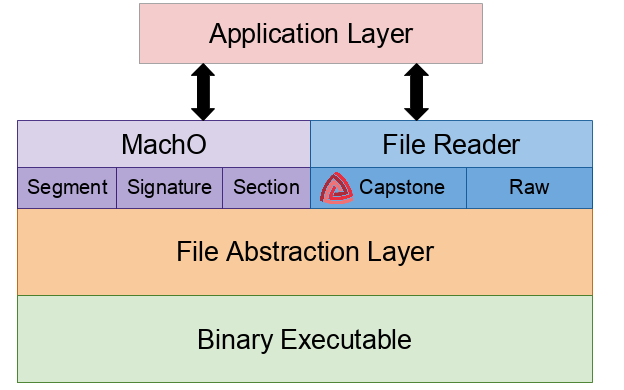
\includegraphics[scale=0.4]{MachoArch1.png}
  \centering
\end{figure}

We can notice that the API is defined by two classes, namely MachO and
FileReader, which together expose functionality to the userspace. The
foundation that these two classes rest on remaines unchanged for now.

Nevertheless, an important change has occured in the archiecture of our
library: the entry point has changed from the MachO class, to the
UniversalBinary class, which is a more general abstraction of a MachO
executable:

\begin{figure}[H]
  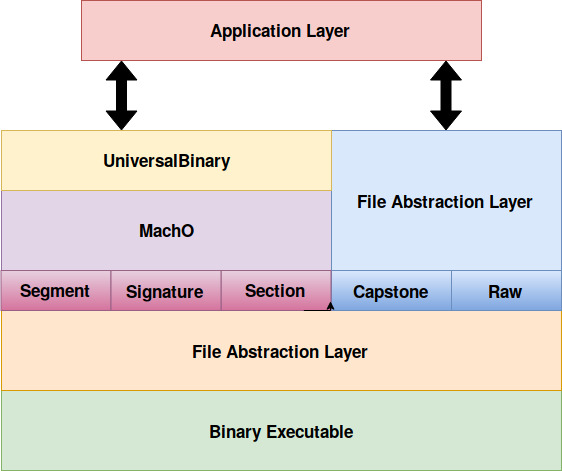
\includegraphics[scale=0.4]{MachoArch2.jpg}
  \centering
\end{figure}

Basically, the UniversalBinary class wraps both the concept of a fat binary,
as well as that of a simple binary (containing code for only one
architecture).

The final API is yet to be defined, even though the current state of the
project has a working fat header and far architecture header parser.


\section{Implementation challenges}
\label{sec:challenges}
% vim: set tw=78 sts=2 sw=2 ts=8 aw et ai:
The main challenge of working on this project was that there is a low amount
of documentation available about the format of a binary file. Adding to this
is the fact that the number of system calls can grow from one kernel version
to another, and the signature marking the start of the table's location
sometimes changes from one kernel version to another. Another challenge to
syscall table extraction is the fact that for some versions of the kernel, the
names of the system calls is also kept in the kernel cache, but on others they
are not.


\section{Lessons learned}
\label{sec:lessons}
% vim: set tw=78 sts=2 sw=2 ts=8 aw et ai:

The binary track of the project yielded concrete progress on the anatomy of a
binary file, especially in the case of Universal Binaries. As a visual
representation, the following image is a very accurate diagram of the
internals of a Fat Binary:

% source: http://www.cocoadev.co.kr/87
\begin{figure}[H]
  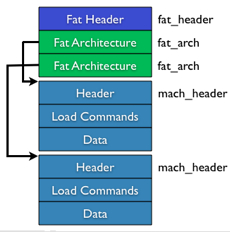
\includegraphics[scale=0.6]{fatBinary.jpg}
  \centering
\end{figure}

There is only one Fat Header (struct fat_header) and at least two Fat
Architectures (struct fat_arch). Generally, the grouping of the Fat Header and
Fat Architectures is called the 'Fat Header', even though that is not entirely
accurate (given the fact that only the struct fat_header should is the
'actual' Fat Header). Such confusion is very frequently encountered.


\section{Current status}
\label{sec:status}
% vim: set tw=78 sts=2 sw=2 ts=8 aw et ai:

Both tracks are very close to fulfilling the first objectives of each track,
therefore we can safely say that nearly one third of the work is almost
achieved. On the Binary Track we have the Universal Binary support that
requires the finishing touches and then it will be merged into the main
branch. The Kernel Track focuses on the syscalls that the kernel provides to
the userspace, and is soon to be finished.


\section{Roadmap}
\label{sec:roadmap}
% vim: set tw=78 sts=2 sw=2 ts=8 aw et ai:


\section{Testing}
\label{sec:testing}
% vim: set tw=78 sts=2 sw=2 ts=8 aw et ai:

So far, testing has been done manually, comparing the outputs of our library
to the outputs of known and validated tools such as otool or objdump. In the
future, there might be efforts of automating the testing process and unit tests
might be introduced.


\section{Further Work}
\label{sec:further}
% vim: set tw=78 sts=2 sw=2 ts=8 aw et ai:

In the next few weeks we will focus on:

\begin{description}
    \item Binary track:
            \begin{description}
                \item Fat binary (universal binary) support
                \item Entitlement signature extraction
            \end{description}
    \item Kernel track:
            \begin{description}
                \item Sandbox profile sandbox extraction
                \item Dump syscall table
            \end{description}
\end{description}


\section{Conclusion}
\label{sec:conclusion}
% vim: set tw=78 sts=2 sw=2 ts=8 aw et ai:

Our work wants to tackle the tehnical challenge posed by the environment 
as well as the fact that there are no open source solutions that would qualify
as better alternatives.


\bibliographystyle{unsrt}
\bibliography{report}

\end{document}
